\documentclass[11pt]{ctexart}
% \documentclass{article}
\textheight 23.5cm \textwidth 15.8cm
%\leftskip -1cm
\topmargin -1.5cm \oddsidemargin 0.3cm \evensidemargin -0.3cm

\usepackage{verbatim}
\usepackage{fancyhdr}
\usepackage{graphicx}
\usepackage{amssymb}
\usepackage{amsmath}
\usepackage{booktabs}
\usepackage{subcaption}
\usepackage{listings}
\usepackage{color}
\usepackage{geometry}


\definecolor{mygreen}{rgb}{0,0.6,0}
\definecolor{mygray}{rgb}{0.5,0.5,0.5}
\definecolor{mymauve}{rgb}{0.58,0,0.82}

\lstset{
  language=Matlab,                % 设定语言为MATLAB
  frame=single,                   % 外围框架
  basicstyle=\footnotesize\ttfamily,   % 基本代码风格
  keywordstyle=\color{blue},      % 关键词风格
  commentstyle=\color{mygreen},   % 注释风格
  stringstyle=\color{mymauve},    % 字符串风格
  numbers=left,                   % 行号位置
  numberstyle=\tiny\color{mygray}, % 行号风格
  stepnumber=1,                   % 行号步长
  numbersep=5pt,                  % 行号与代码间隔
  backgroundcolor=\color{white},  % 代码背景色
  showspaces=false,               % 不显示空格
  showstringspaces=false,         % 不显示字符串中的空格
  showtabs=false,                 % 不显示制表符
  tabsize=4,                      % 制表符宽度
  captionpos=b,                   % 标题位置
  breaklines=true,                % 自动换行
  breakatwhitespace=false,        % 仅在空格处换行
  escapeinside={\%*}{*)},         % 可以添加LaTeX内容
}


\ctexset {
     section/format    += \sffamily\raggedright,
     subsection/format += \fbox,
}

\title{FEM Code Report5}
\author{SA24229016 王润泽}

\begin{document}
\maketitle

\section{Introduction}
编写程序求解 $ \Omega=[0,1]\times [0,1] $定义域范围的 Dirichlet边值问题:
\begin{equation}
     \begin{aligned}
         -\nabla^2 u &= f \quad \text{in } \Omega, \\
         u &= 0 \quad \text{on } \partial \Omega.
     \end{aligned}
\end{equation}
有限元空间选取为分段连续二次多项式空间 $ V_h $
\begin{equation}
  V_h = \{ v_h \in C(\Omega) : v_h|_k \in P^2(k), \forall k \in \mathcal{T}_h, v_h|_{\partial \Omega} = 0 \}.
\end{equation}

要求,准确解为 $ u(x,y) = (x-1)\sin(x)(y-1)\sin(y) $。

\section{Algorithm}
\subsection{Variational Formulation}
首先将 Dirichlet边值问题转化为如下变分问题:

定义双线性形式:

$$ a(u,v) = \int_{\Omega} \nabla u \cdot \nabla v \, dx dy $$ 

线性形式 
$$ L(v) = \int_{\Omega} f v \, dx dy .$$

那么问题(1)的变分问题为:求 $ u \in V = \{ v \in H^2(\Omega) : v|_{\partial \Omega} = 0 \} $ ,使得对于所有 $ v \in V $ ,有:
\begin{equation}
     a(u,v) = L(v).
\end{equation}

\subsection{Finite Element Space}
为了进行数值求解,选择一个分段连续二次多项式空间 $ V_h \subset V$进行求解。变分问题(3)的离散化形式为:Find $ u_h \in V_h $ such that
\begin{equation}
  a(u_h,v_h) = L(v_h), \quad \forall v_h \in V_h.
\end{equation}

\subsubsection{Triangulation}
首先,对于二维有限元问题,我们采用三角剖分的方法,将二维区域剖分为三角形网格集合 $ \mathcal{T}_h=\{k_i\} $ ,每个三角形上定义一个局部的有限元空间。

考虑到我们采取的是分段连续二次多项式空间 $ V_h $ ,因此我们需要在每个局部三角形上定义一个二次多项式空间 $ P^2(k) $,
\begin{equation}
  P^2(k) = \text{span}\{1,x,y,x^2,xy,y^2\}.
\end{equation}

共有6个基函数,因此我们选择三角形的3个顶点和3个边中点作为基函数的支撑点,如图1所示.
\begin{figure}[htbp]
  \centering
  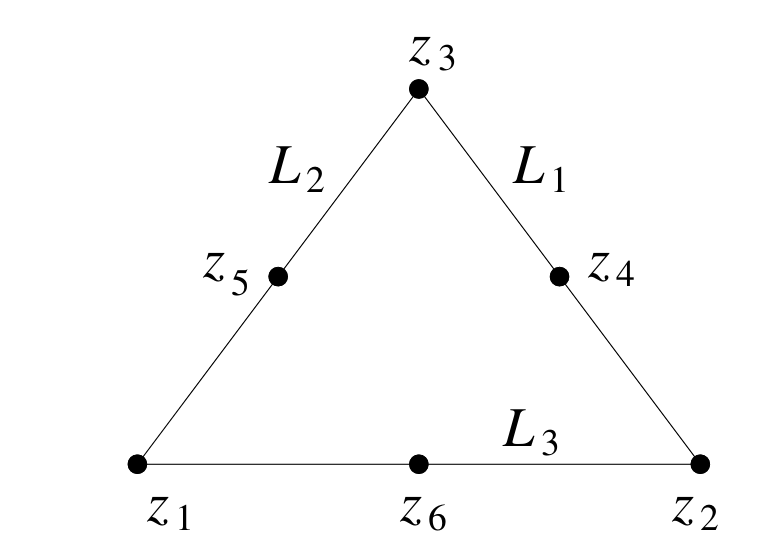
\includegraphics[width=0.3\textwidth]{quadratic.png}
  \caption{quadratic basis function}
  \label{fig: quadratic}
\end{figure}



\subsubsection{Local Basis Function}
对于每个三角形 $ k\in \mathcal{T}_h $ ,由其三个顶点定义 $ P_1,P_2,P_3 $ 和三个边中点 $ P_4,P_5,P_6 $,我们选取一个分段二次多项式空间作为局部的基函数 $ u(x,y) $:
\begin{equation}
      u(x,y) = a_1 + a_2 x + a_3 y + a_4 x^2 + a_5 xy + a_6 y^2,
\end{equation}
在三角形顶点处满足 $ u(P_i) = u_i $ ,其中 $ P_i $ 为三角形顶点和边中点的全局坐标,$ u_i $ 为顶点处的值,$ i=1,2,...,6 $,$ u_i $ 即为待求解的值。此时对于每个点的基函数 $ N_i(x,y) $ 满足:
\begin{equation}
  N_i(P_j) = \delta_{ij},
\end{equation}

容易得到,基函数的表达式为:
\begin{gather}
  N_1(x,y) = \lambda_1(2\lambda_1-1)\\
  N_2(x,y) = \lambda_2(2\lambda_2-1)\\
  N_3(x,y) = \lambda_3(2\lambda_3-1)\\
  N_4(x,y) = 4\lambda_2\lambda_3\\
  N_5(x,y) = 4\lambda_3\lambda_1\\
  N_6(x,y) = 4\lambda_1\lambda_2
\end{gather}
其中,$ \lambda_i $ 为重心坐标函数,满足:
\begin{equation}
  \begin{aligned}
    &\lambda_i(x,y) = \frac{1}{2\Delta_k} (a_i x + b_i y + c_i)\\
    &a_i = y_j-y_m, \quad b_i = x_m-x_j, \quad c_i = x_j y_m - x_m y_j
  \end{aligned}
\end{equation}
$ \Delta_k $ 为三角形面积, $ i,j,m $ 为三角形顶点编号,下标符合轮换对称性,且有 $ \lambda_1 + \lambda_2 + \lambda_3 = 1 $。

\subsubsection{Stiffness Matrix}
对于每个单位三角形 $ \hat{k} $ 区域内的基函数 $ \hat{N}_i(\lambda_1,\lambda_2) $ 求偏导数,根据双线性泛函$ a(\cdot,\cdot) $ 的定义,对于单位三角形局部刚度矩阵 $ \hat{A}_k $ 可以写成:

\begin{equation}
    \left(\hat{\mathbf{A}}_k\right)_{ij} = \int_{\hat{k}} \nabla \hat{N_i} \cdot \nabla \hat{N_j} \, d\lambda_1 d\lambda_2\\
\end{equation}

\begin{equation}
  \hat{\mathbf{A}}_k =   \begin{bmatrix}
    \frac{1}{2}& 0 & \frac{1}{6} &  0 & -\frac{2}{3} & 0\\
    0 & \frac{1}{2} & \frac{1}{6} &  -\frac{2}{3} & 0 & 0\\
    \frac{1}{6} & \frac{1}{6} & 1 & -\frac{2}{3} & -\frac{2}{3} & 0\\
    0 & -\frac{2}{3} & -\frac{2}{3} &  \frac{8}{3} & 0 & -\frac{4}{3}\\
    -\frac{2}{3} & 0 & -\frac{2}{3} & 0 & \frac{8}{3} & -\frac{4}{3}\\
    0 & 0 & 0 &  -\frac{4}{3} & -\frac{4}{3} & \frac{8}{3}\\

  \end{bmatrix}
\end{equation}

转换到全局坐标系下时,如果我们三角化过程满足,每个三角形 $ k $ 是标准直角三角形,且三角形的面积为 $ \Delta_k = \frac{h^2}{2} $,那么有:
\begin{gather*}
    \frac{\partial}{\partial x} = \frac{1}{h}\frac{\partial}{\partial \lambda_1},\\  
    \frac{\partial}{\partial y} = \frac{1}{h}\frac{\partial}{\partial \lambda_2}\\
    \left|\frac{\partial(x,y)}{\partial(\lambda_1,\lambda_2)}\right|= h^2
\end{gather*}

此时,我们可以得到局部刚度矩阵 $ A_k $ :
\begin{equation}
  \int_k \nabla N_i \cdot \nabla N_j \, dx dy =\int_{\hat{k}} \nabla \hat{N_i} \cdot \nabla \hat{N_j} \, d\lambda_1 d\lambda_2
\end{equation}
即:
\begin{equation}
  \mathbf{A}_k = \hat{\mathbf{A}}_k
\end{equation}

在构造全局刚度矩阵时,只需将局部刚度矩阵 $ \mathbf{A}_k $ 按照顶点索引的位置加到全局刚度矩阵 $ \mathbf{A} $ 的对应位置上即可。比如,对于三角形 $ k $ 的局部刚度矩阵的元素 $ a_{12} $ 对应的分别是 $ u_1^k $ 和 $ u_2^k $ ,那么只要找到顶点 $ P_1^k $ 和 $ P_2^k $ 的全局索引,将 $ a_{12} $ 加到 全局刚度$ \mathbf{A} $ 的对应位置上即可。

\subsubsection{Load Vector}
同理,对于单位三角形 $ \hat{k} $ 区域内的基函数 $ \hat{N}_i(\lambda_1,\lambda_2) $ ,根据线性泛函$ L(\cdot) $ 的定义,对于单位三角形局部载荷向量 $ \hat{\mathbf{b}}_k $ 可以写成:
\begin{equation}
  \begin{aligned}
    (\hat{\mathbf{b}}_k)_i &= \int_{\hat{k}} f \hat{N}_i \, d\lambda_1 d\lambda_2\\
    &\approx f(P_i) \int_{\hat{k}} \hat{N}_i \, d\lambda_1 d\lambda_2
  \end{aligned}
\end{equation}

\begin{equation}
  \hat{\mathbf{b}}_k = \begin{bmatrix}
    f(P_1)\\
    f(P_2)\\
    f(P_3)\\
    f(P_4)\\
    f(P_5)\\
    f(P_6)
  \end{bmatrix}\otimes
  \begin{bmatrix}
    0\\
    0\\
    0\\
    1/6\\
    1/6\\
    1/6
  \end{bmatrix}
\end{equation}

转换到全局坐标系下时有:
\begin{equation}
    b_k = \hat{b}_k \left|\frac{\partial(x,y)}{\partial(\lambda_1,\lambda_2)}\right|= \hat{b}_k h^2
\end{equation}


\section{Results}
(1). 求解出满足方程的 $ f(x,y) $
%-((2*cos(x) - (-1+x) .* sin(x)) .* (y-1) .* sin(y) + (x-1) .* sin(x) .* (2*cos(y) - (-1+y).*sin(y)));
\begin{equation}
  \begin{aligned}
    f(x,y) = &((x-1) \cdot \sin(x)-2\cos(x)) \cdot (y-1) \cdot \sin(y)\\
    &((y-1)\cdot\sin(y)-2\cos(y))\cdot(x-1) \cdot \sin(x)
  \end{aligned}
\end{equation}

(2).对区域采用三角形网格剖分 $ \mathcal{T}_h $ ,给出总网格个数、对应的内部结点和边界结点的个数:

对于整个空间,得到三角网格面元单元数为 $ 2N^2 $,内部顶点数为 $ (2N-1)^2 $,边界顶点数为 $ 8N$,

(3). 输出初始网格的结点编号和三角单元的编号方式:如图2所示.
\begin{figure}[htbp]
      \centering
      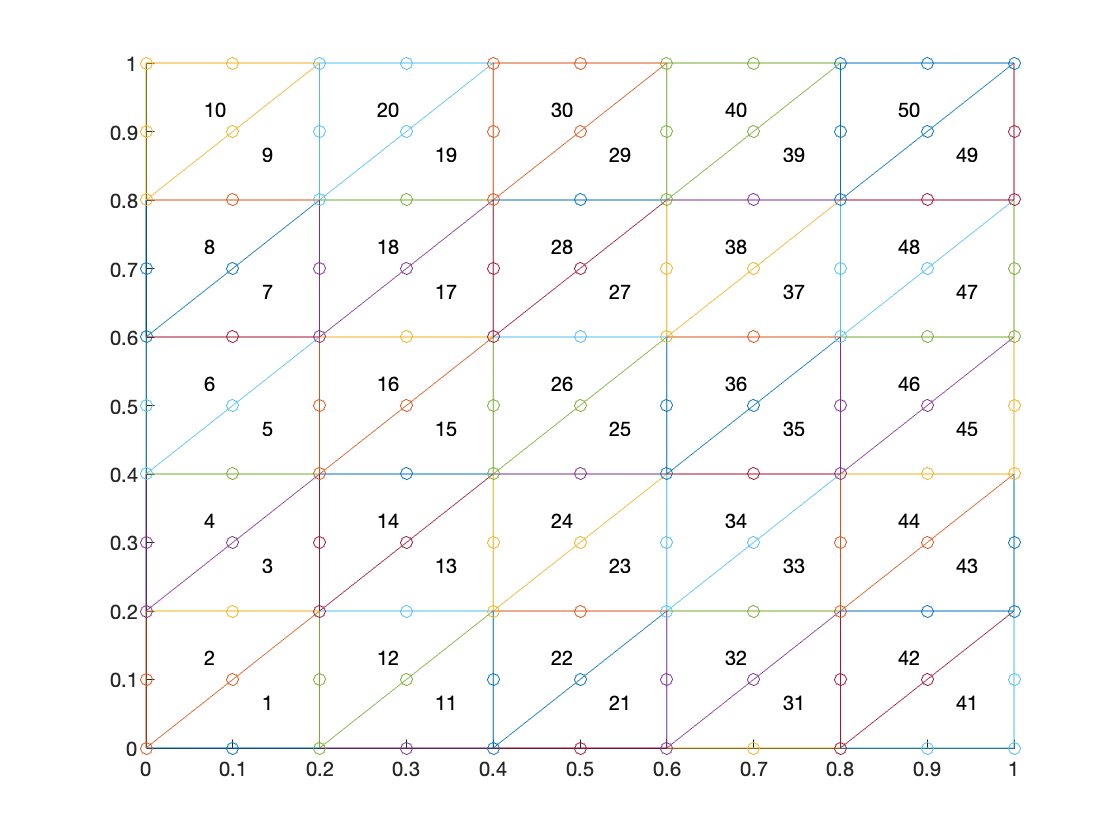
\includegraphics[width=0.4\textwidth]{triangulation.png}
      \caption{Triangulation}
      \label{fig:triangulation}
\end{figure}

(4). 输出初始网格对应的刚度矩阵的非零元的图像: 如图3所示.
\begin{figure}[htbp]
  \centering
  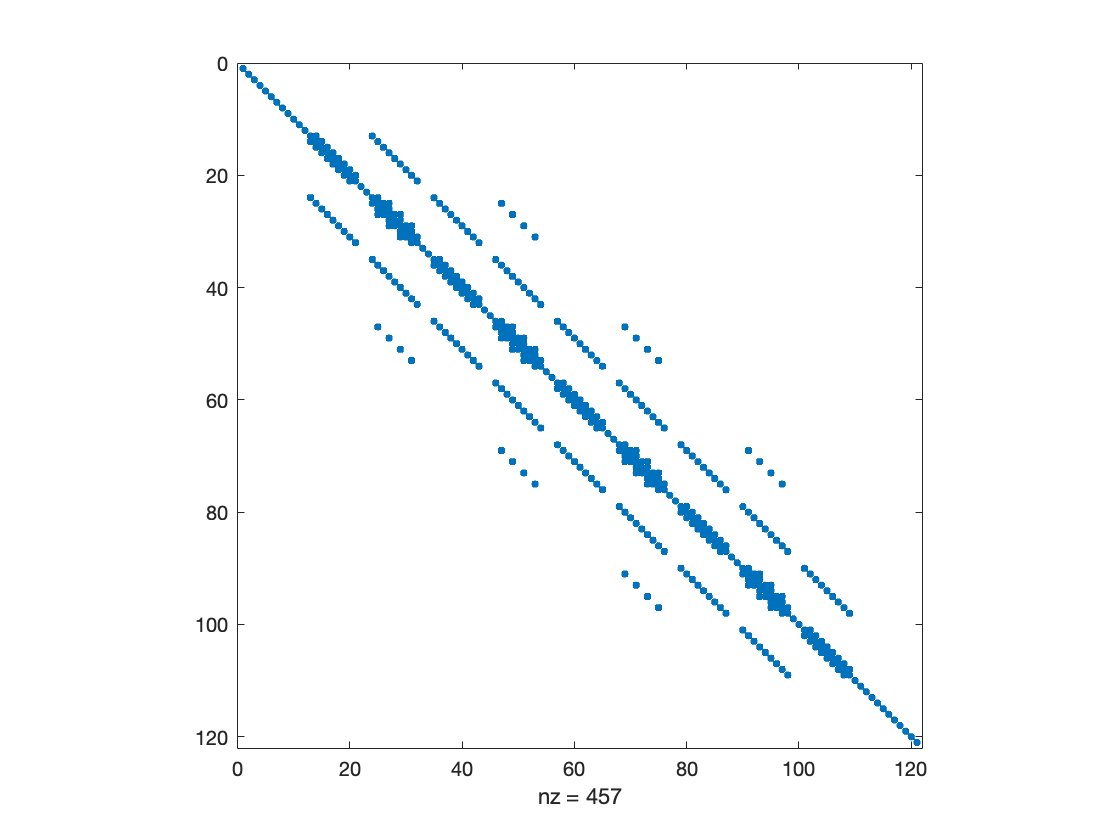
\includegraphics[width=0.4\textwidth]{matrix.png}
  \caption{Stiffness Matrix}
  \label{fig:stiffness}
\end{figure}

(6). 求解有限元问题,测试程序,并计算 $ L^2,H^1 $ 误差和误差阶。
\begin{table}[htbp]
  \centering
  \begin{tabular}{|c|c|c|cc|cc|}
    \toprule
    网格总数 & 总内部结点数 & 总边界点数& \multicolumn{1}{c}{$L^2$ error} & \multicolumn{1}{c|}{order} & \multicolumn{1}{c}{$H^1$ error} & \multicolumn{1}{c|}{order} \\
    \midrule
    200 & 361 & 80     & 9.72E-07 &       & 8.04E-05 &       \\
    800 & 1521 & 160   & 9.61E-08 & 3.338 & 1.80E-05 & 2.163 \\
    3200 & 6241 & 320  & 1.01E-08 & 3.253 & 4.19E-06 & 2.100 \\
    12800& 25281 & 640 & 1.12E-09 & 3.169 & 1.01E-06 & 2.057 \\
    \bottomrule
  \end{tabular}%
  \label{tab:error}%
\end{table}%

误差分析:因为选择了2次的Lagrange 单元,那么它的插值误差是$O(h^3)$的,对于导数的误差是$O(h^2)$ 这和我们期望的误差阶是相同的。

\end{document}